\chapter{}

\section{Sub-heading}

Vivamus vitae massa adipiscing est lacinia sodales. Donec metus massa, mollis vel, tempus placerat, vestibulum condimentum, ligula. Nunc lacus metus, posuere eget, lacinia eu, varius quis, libero. Aliquam nonummy adipiscing augue. Lorem ipsum dolor sit amet, consectetuer adipiscing elit. Maecenas porttitor congue massa. Fusce posuere, magna sed pulvinar ultricies, purus lectus malesuada libero, sit amet commodo magna eros quis urna. Nunc viverra imperdiet enim.

% This is an example of a simple table
\begin{table}
\centering
\begin{tabular}{|c|c|c|}
\hline
1-2-3 & yes & no \\
\hline
Multiplan & yes & yes \\
\hline
Wordstar & no & no \\
\hline
\end{tabular}
\caption{This is an example of a simple table.}
\end{table}

Fusce est. Vivamus a tellus. Pellentesque habitant morbi tristique senectus et netus et malesuada fames ac turpis egestas. Proin pharetra nonummy pede. Mauris et orci. Aenean nec lorem. In porttitor.\par

Donec laoreet nonummy augue. Suspendisse dui purus, scelerisque at, vulputate vitae, pretium mattis, nunc. Mauris eget neque at sem venenatis eleifend. Ut nonummy. Fusce aliquet pede non pede. Suspendisse dapibus lorem pellentesque magna. Integer nulla. Donec blandit feugiat ligula.\par


% This is an example of a more complex table
\begin{table}
\centering
\begin{tabular}{|ccccc|}
\hline
\textbf{Mitre} & \textbf{Enchantress} & \textbf{Hagstrom} &
\textbf{Atlantica} & \textbf{Martinez} \\
\hline
Arabic & Spicebush & Sapient & Chaos & Conquer \\
Jail & Syndic & Prevent & Ballerina & Canker \\
Discovery & Fame & Prognosticate & Corroborate & Bartend \\
Marquis & Regal & Accusation & Dichotomy & Soprano \\
Indestructible  & Porterhouse & Sofia & Cavalier & Trance \\
Leavenworth & Hidden & Benedictine & Vivacious & Utensil \\
\hline
\end{tabular}
\caption{This is an example of a slightly more complex table}
\end{table}

Donec hendrerit, felis et imperdiet euismod, purus ipsum pretium metus, in lacinia nulla nisl eget sapien. Donec ut est in lectus consequat consequat. Etiam eget dui. Aliquam erat volutpat. Sed at lorem in nunc porta tristique. Proin nec augue. Quisque aliquam tempor magna. Pellentesque habitant morbi tristique senectus et netus et malesuada fames ac turpis egestas.\par

\begin{figure}
\caption{Example of a basic figure title}
%Use the scale parameter to size the image
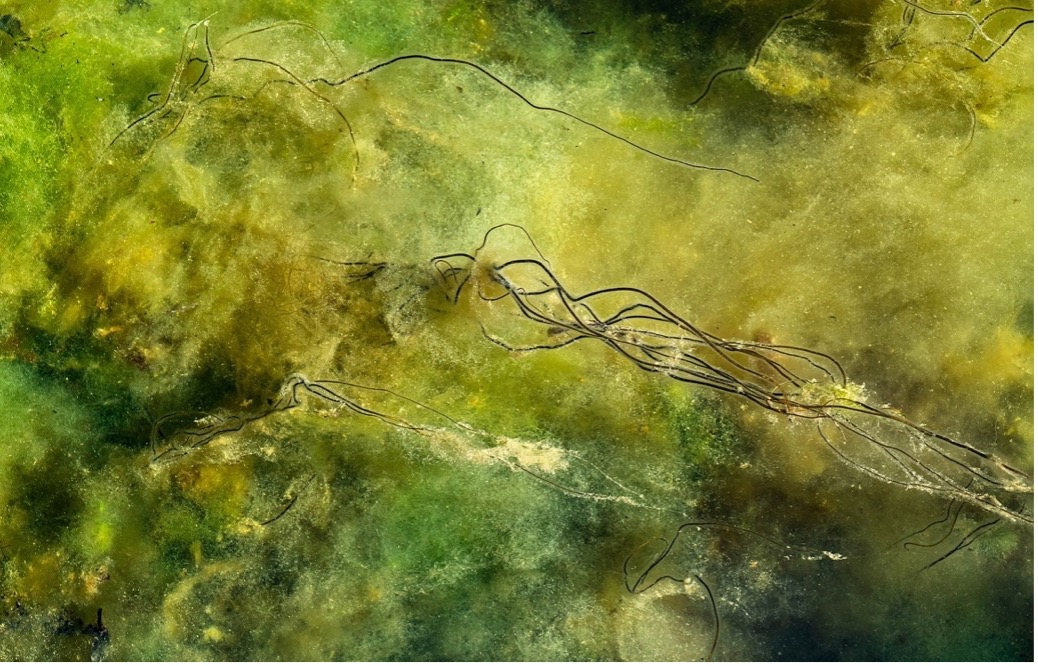
\includegraphics[scale=.45]{Picture2}

% here is an alternate way to scale images based on specific sizes
%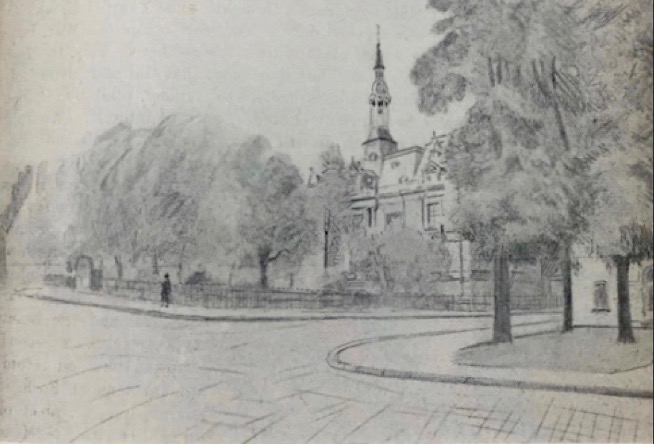
\includegraphics[width=5cm, height=4cm]{Picture1}
 \emph{This is an example of an image caption or description}
\end{figure}

Nunc ac magna. Maecenas odio dolor, vulputate vel, auctor ac, accumsan id, felis. Pellentesque cursus sagittis felis. Pellentesque porttitor, velit lacinia egestas auctor, diam eros tempus arcu, nec vulputate augue magna vel risus. Cras non magna vel ante adipiscing rhoncus. Vivamus a mi. Morbi neque. Aliquam erat volutpat. Integer ultrices lobortis eros. Pellentesque habitant morbi tristique senectus et netus et malesuada fames ac turpis egestas.\par

Proin semper, ante vitae sollicitudin posuere, metus quam iaculis nibh, vitae scelerisque nunc massa eget pede. Sed velit urna, interdum vel, ultricies vel, faucibus at, quam. Donec elit est, consectetuer eget, consequat quis, tempus quis, wisi. In in nunc. Class aptent taciti sociosqu ad litora torquent per conubia nostra, per inceptos hymenaeos. Donec ullamcorper fringilla eros. Fusce in sapien eu purus dapibus commodo.\par


% This is an example of figure drawn using code
\begin{figure}\centering
\parbox{.4\textwidth}{\centering
\begin{picture}(70,70)
\put(0,50){\framebox(20,20){}}
\put(10,60){\circle*{7}}
\put(50,50){\framebox(20,20){}}
\put(60,60){\circle*{7}}
\put(20,10){\line(1,0){30}}
\put(20,10){\line(-1,1){10}}
\put(50,10){\line(1,1){10}}
\end{picture}
\caption{Donec eu condimentum.}}
\hfill
\parbox{.4\textwidth}{\centering
\begin{picture}(70,70)
\put(0,50){\framebox(20,20){}}
\put(10,60){\circle*{7}}
\put(50,50){\framebox(20,20){}}
\put(60,60){\circle*{7}}
\put(20,10){\line(1,0){30}}
\put(20,10){\line(-1,-1){10}}
\put(50,10){\line(1,-1){10}}
\end{picture}
\caption{Quisque dapibus dignissim.}}
\end{figure}

Nam ac viverra dolor, sed pulvinar justo. Nullam orci est, ultrices non justo vel, euismod aliquet ligula. Cras semper, purus sed pharetra rhoncus, metus mauris ultricies odio, non sodales odio est finibus velit.

% Block quote example
\begin{quote}
This is an example of a block quote. Donec id mi at nulla tempor tincidunt a sit amet mi. Vivamus pulvinar dolor felis. Mauris in tellus accumsan, pellentesque lacus eu, aliquet lectus. Suspendisse felis nulla, scelerisque at maximus ut, mollis laoreet nisi. Pellentesque pulvinar libero pharetra dolor blandit pulvinar. Proin dapibus sodales velit ac rhoncus.
\end{quote}

Donec id mi at nulla tempor tincidunt a sit amet mi. Vivamus pulvinar dolor felis. Mauris in tellus accumsan, pellentesque lacus eu, aliquet lectus. Suspendisse felis nulla, scelerisque at maximus ut, mollis laoreet nisi. Pellentesque pulvinar libero pharetra dolor blandit pulvinar. Proin dapibus sodales velit ac rhoncus. Integer lacinia justo et enim porta porta. Praesent odio velit, ultrices interdum tortor in, consectetur bibendum dolor.

% This is an example of how to use footnotes
This is an example of a footnote.\footnote{This is the text that will appear in the footnote} Pellentesque libero lectus, tristique ac, consectetuer sit amet, imperdiet ut, justo. Sed aliquam odio vitae tortor. Proin hendrerit tempus arcu. In hac habitasse platea dictumst. Suspendisse potenti.


\begin{theorem}
\tolerance=10000\hbadness=10000
This is an example of how to use the theorem environment.
\end{theorem}


% Here as another example of a figure that has been drawn progammatically
\begin{figure}
\parbox{1\textwidth}{\centering
\begin{picture}(90,50)
  \put(0,0){\circle*{5}}
  \put(0,0){\vector(1,1){31.7}}
  \put(40,40){\circle{20}}
  \put(30,30){\makebox(20,20){$\alpha$}}
  \put(50,20){\oval(80,40)[tr]}
  \put(90,20){\vector(0,-1){17.5}}
  \put(90,0){\circle*{5}}
\end{picture}
\caption{ Here we see an example of a figure which has been drawn programatically using \LaTeX}}
\end{figure}

\begin{sidewaystable}
\centering
\begin{tabular}{|ccccc|}
\hline
\textbf{Mitre} & \textbf{Enchantress} & \textbf{Hagstrom} &
\textbf{Atlantica} & \textbf{Martinez} \\
\hline
Arabic & Spicebush & Sapient & Chaos & Conquer \\
Jail & Syndic & Prevent & Ballerina & Canker \\
Discovery & Fame & Prognosticate & Corroborate & Bartend \\
Marquis & Regal & Accusation & Dichotomy & Soprano \\
Indestructible  & Porterhouse & Sofia & Cavalier & Trance \\
Leavenworth & Hidden & Benedictine & Vivacious & Utensil \\
\hline
\end{tabular}
\caption{Here we have an example of a table that has been set in landscape}
\end{sidewaystable}


\begin{itemize}
\item This is an example of a bulleted list.
\item Praesent vestibulum mi turpis, vitae ultricies diam porttitor non.
\item Morbi sed vulputate nibh, ac iaculis odio.
\item Mauris ac risus eget eros ornare.
\item Proin quis tellus non velit posuere pulvinar.
\item Vestibulum tincidunt tempor hendrerit.
\item Praesent ornare imperdiet diam, sit amet laoreet.
\end{itemize}


\begin{enumerate}
\item This is an example of a numbered list.
\item Praesent vestibulum mi turpis, vitae ultricies diam porttitor non.
\item Morbi sed vulputate nibh, ac iaculis odio.
\item Mauris ac risus eget eros ornare.
\item Proin quis tellus non velit posuere pulvinar.
\item Vestibulum tincidunt tempor hendrerit.
\item Praesent ornare imperdiet diam, sit amet laoreet.
\end{enumerate}

\section{Math Examples}

Here we see an equation placed within an equation environment\par

\section{Math Examples}

Here we see an equation placed within an equation environment\par
\begin{equation}
cos (2\theta) = {\cos^2}\theta - \sin^2 \theta
\end{equation}

Here we see an equation which has not been placed in an equation environment\par
$
\lim\limits_{x \to \infty} \exp(-x) = 0
$

Here we have several more math examples\par
$
k_{n+1} = n^2 + k_n^2 - k_{n-1}
$

$
f(n) = n^5 + 4n^2 + 2 |_{n=17}
$

$
\frac{n!}{k!(n-k)!} = {n}{k}
$

$\frac{\frac{1}{x}+\frac{1}{y}}{y-z}$

\begin{equation}
\frac{
    \begin{array}[b]{r}
      \left( x_1 x_2 \right)\\
      \times \left( x'_1 x'_2 \right)
    \end{array}
  }{
    \left( y_1y_2y_3y_4 \right)
  }
\end{equation}

$\sqrt{\frac{a}{b}}$

$\sqrt[n]{1+x+x^2+x^3+\dots+x^n}$

$\sum_{i=1}^{10} t_i$

$\displaystyle\sum_{i=1}^{10} t_i$

$P\left(A=2\middle|\frac{A^2}{B}>4\right)$






